\chapter{Arhitektura i dizajn sustava}
		
		\textbf{\textit{dio 1. revizije}}\\

		\textit{ Potrebno je opisati stil arhitekture te identificirati: podsustave, preslikavanje na radnu platformu, spremišta podataka, mrežne protokole, globalni upravljački tok i sklopovsko-programske zahtjeve. Po točkama razraditi i popratiti odgovarajućim skicama:}
	\begin{itemize}
		\item 	\textit{izbor arhitekture temeljem principa oblikovanja pokazanih na predavanjima (objasniti zašto ste baš odabrali takvu arhitekturu)}
		\item 	\textit{organizaciju sustava s najviše razine apstrakcije (npr. klijent-poslužitelj, baza podataka, datotečni sustav, grafičko sučelje)}
		\item 	\textit{organizaciju aplikacije (npr. slojevi frontend i backend, MVC arhitektura) }		
	\end{itemize}

	
		

		

				
		\section{Baza podataka}
			
			\textbf{\textit{dio 1. revizije}}\\
			
		\textit{Potrebno je opisati koju vrstu i implementaciju baze podataka ste odabrali, glavne komponente od kojih se sastoji i slično.}
		
			\subsection{Opis tablica}
			
					    \textbf{ Korisnik}
		    \item Ovaj entitet sadržava sve važne informacije o korisniku aplikacije. Sadrži atribute: ID${\_}$Korisnika ,ime ,prezime,
		     email, lozinku,ulogu,aktivan,token te duljinu i sirinu. Ovaj entitet je u vezi \emph{One-to-Many} s entitom Izvršavanje preko atributa ID${\_}$Korisnika, u vezi \emph{One-to-Many} s entitetom Zahtjev preko atributa ID${\_}$Korisnika,u vezi s Lokacijom prkeo atributa duljina i širina, u vezi s entitetom Kandidiranje preko atributa ID${\_}$Korisnika te u vezi \emph{One-to-Many} s entitetom Ocjenjivanje preko atributa ID${\_}$Korisnika gdje korisnik ima dvije uloge. 
				
				\begin{longtabu} to \textwidth {|X[6, l]|X[6, l]|X[20, l]|}
					
					\hline \multicolumn{3}{|c|}{\textbf{Korisnik}}	 \\[3pt] \hline
					\endfirsthead
					
					\hline \multicolumn{3}{|c|}{\textbf{Korisnik }}	 \\[3pt] \hline
					\endhead
					
					\hline 
					\endlastfoot
					
					\cellcolor{LightGreen}ID${\_}$Korisnik & SERIAL	& jedinstveni identifikator korisnika 	 	\\ \hline
					ime & VARCHAR	&  ime korisnika	\\ \hline 
					prezime & VARCHAR	& prezime korisnika 		\\ \hline
					email & VARCHAR & e-mail adresa korisnika  \\ \hline 
					lozinka	& VARCHAR & hash lozinke 	\\ \hline 
					uloga	& VARCHAR & uloga korisnika (administrator ili registrirani korisnik)  	\\ \hline 
					aktivan & BOOLEAN & status korisnika \\ \hline
					token & VARCHAR & ??? \\ \hline
					duljina & NUMERIC & geografska duljina \\ \hline
					
					\cellcolor{LightBlue} sirina	& NUMERIC & geografska širina  \\ \hline 
					
					
				\end{longtabu}
			    \textbf{ Zahtjev}
		    \item Ovaj entitet sadržava sve važne informacije o korisnikovu zahtjevu. Sadrži atribute: ID${\_}$Zahtjev ,opis,datum,vrijeme,status,brojMobitela,ID${\_}$Autora,duljinu i širinu.Ovaj entitet je u vezi s entitom Lokacija preko atributa sirina i duljina,također u vezi  s entitetom Izvrsavanje preko atributa ID${\_}$Zahtjev te u vezi \emph{Many-to-One} s entitetom Korisnik preko ID${\_}$Korisnika.  
			
				\begin{longtabu} to \textwidth {|X[6, l]|X[6, l]|X[20, l]|}
					
					\hline \multicolumn{3}{|c|}{\textbf{Zahtjev}}	 \\[3pt] \hline
					\endfirsthead
					
					\hline \multicolumn{3}{|c|}{\textbf{Zahtjev }}	 \\[3pt] \hline
					\endhead
					
					\hline 
					\endlastfoot
					
					\cellcolor{LightGreen}ID${\_}$Zahtjev & SERIAL	&  jedinstveni identifikator korisnika	 	\\ \hline
					opis & VARCHAR	& opis zahtjeva 		\\ \hline 
					datum & DATE	& datum do kada se treba izvršiti zahtjev  		\\ \hline
					vrijeme & TIME & vrijeme do kada se treba izvršiti zahtjev \\ \hline 
					status	& VARCHAR & status zahtjeva  	\\ \hline
					brojMobitela & VARCHAR & broj mobitela autora zahtjeva? \\ \hline
					ID${\_}$Autora & SERIAL & jedinstveni identifikator korisnika(autora zahtjeva) \\ \hline
					duljina & NUMERIC & geografska duljina \\ \hline
					\cellcolor{LightBlue} sirina & NUMERIC & geografsk širina    	\\ \hline 
					
					
				\end{longtabu}
						    \textbf{ Lokacija}
		    \item Ovaj entitet sadržava sve važne informacije o lokaciji. Sadrži atribute: geografsku duljinu i geografsku širinu, ime drzave, naselje te adresu.Ovaj entitet je u vezi s entitom Zahtjev preko atributa sirina i duljina,također u vezi  s entitetom Korisnikom preko atributa duljina i sirina te u vezi \emph{One-to-Many} s entitetom Kandidatura preko duljina i sirina. 
			
				\begin{longtabu} to \textwidth {|X[6, l]|X[6, l]|X[20, l]|}
					
					\hline \multicolumn{3}{|c|}{\textbf{Lokacija}}	 \\[3pt] \hline
					\endfirsthead
					
					\hline \multicolumn{3}{|c|}{\textbf{Lokacija }}	 \\[3pt] \hline
					\endhead
					
					\hline 
					\endlastfoot
					
					\cellcolor{LightGreen}duljina & NUMERIC	& geografska dužina \\ \hline
					sirina & NUMERIC & geografska sirina \\ \hline
					drzava & VARCHAR	& naziv države 		\\ \hline
					naselje & VARCHAR & naziv naselja  \\ \hline 
					\cellcolor{LightBlue} adresa	& VARCHAR & adresa na kojoj treba odraditi zahtjev	\\ \hline 	
					
				\end{longtabu}
			
			
		    \textbf{ Izvršavanje}
		    \item Ovaj entitet sadržava sve važne informacije o izvršiteljima zahtjeva i podacima koji im omogućavaju samo izvršavanje. Sadrži atribute: ID zahtjeva koji izvršavaju, ID izvršitelja, primljena obavijest sa nužnim podacima o autoru, ocjena i komentar. Ovaj entitet je u vezi \emph{Many-to-One} sa korisnikom preko atributa ID Izvršitelja i u vezi \emph{One-to-One} sa entitetom Zahtjev preko atributa ID Zahtjev.

				\begin{longtabu} to \textwidth {|X[6, l]|X[6, l]|X[20, l]|}
					
					\hline \multicolumn{3}{|c|}{\textbf{Izvršavanje}}	 \\[3pt] \hline
					\endfirsthead
					
					\hline \multicolumn{3}{|c|}{\textbf{Aut${\_}$Zahtj${\_}$Izvr}}	 \\[3pt] \hline
					\endhead
					
					\hline 
					\endlastfoot
					
					\cellcolor{LightGreen}ID${\_}$Zahtjev & INT	& jedinstveni identifikator zahtjeva 	\\ \hline
					\cellcolor{LightBlue}ID${\_}$Autor & INT	& jedinstveni identifikator autora zahtjeva 	\\ \hline
					\cellcolor{LightBlue}ID${\_}$Izvrsitelj & SERIAL	& jedinstveni identifikator izvršitelja zahtjeva  	\\ \hline
				
					
					
				\end{longtabu}
			\textbf{ Kandidatura}
		    \item Ovaj entitet sadržava sve važne informacije o kandidaturi za korisnika godine. Sadrži atribute: godina kandidature, geografska duljina i širina. Ovaj entitet je u vezi \emph{Many-to-One} sa entitetom Kandidiranje preko atributa godina kandidature, geografska duljina i širina i u vezi \emph{Many-to-One} sa Lokacijom preko atributa geografska duljina i širina.

				\begin{longtabu} to \textwidth {|X[7, l]|X[6, l]|X[20, l]|}
					
					\hline \multicolumn{3}{|c|}{\textbf{Kandidatura}}	 \\[3pt] \hline
					\endfirsthead
					
					\hline \multicolumn{3}{|c|}{\textbf{Kandidatura}}	 \\[3pt] \hline
					\endhead
					
					\hline 
					\endlastfoot
					
					\cellcolor{LightGreen}ID${\_}$Kandidatura & SERIAL	& jedinstveni identifikator kandidature 	\\ \hline
					godina & INT & godina kandidature  \\ \hline 
					\cellcolor{LightBlue}ID${\_}$Korisnik & INT	& jedinstveni identifikator korisnika 	\\ \hline
					
				\end{longtabu}
				
				\textbf{Kandidiranje}
		    \item Ovaj entitet sadržava sve važne informacije o korisniku koji se kandidira za korisnika godine. Sadrži atribute: ID korisnika, godina kandidature, geografska duljina i širina. Ovaj entitet je u vezi \emph{One-to-Many} sa entitetom Kandidatura preko atributa godina kandidature, geografska duljina i širina te u vezi \emph{One-to-One} sa entitetom Korisnik preko atributa ID Korisnika.
		    \newline
		        \textbf{Ocjenjivanje}
		    \item Ovaj entitet sadržava sve važne informacije o međusobnom ocjenjivanju korisnika. Sadrži atribute: ID ocjenjenog korisnika te ID ocjenjivača, ocjena i komentar. Ovaj entitet je u vezi \emph{Many-to-One} sa entitetom Korisnik preko atributa ID ocjenjenog korisnika i ID ocjenjivača.
				\begin{longtabu} to \textwidth {|X[6, l]|X[6, l]|X[20, l]|}
					
					\hline \multicolumn{3}{|c|}{\textbf{Ocjena}}	 \\[3pt] \hline
					\endfirsthead
					
					\hline \multicolumn{3}{|c|}{\textbf{Ocjena }}	 \\[3pt] \hline
					\endhead
					
					\hline 
					\endlastfoot
					
					\cellcolor{LightGreen}ID${\_}$Ocjenitelj & INT	& jedinstveni identifikator ocjenitelja 	\\ \hline
					\cellcolor{LightGreen}ID${\_}$Ocjenjeni & INT	& jedinstveni identifikator ocjenjenog 	\\ \hline
					ocjena & INT	&  ocjena usluge		\\ \hline 
					komentar & VARCHAR	& komentar ocjenitelja 		\\ \hline
					
					
					
				\end{longtabu}
		
		
			\subsection{Dijagram baze podataka}
			
			%unos slike
			\begin{figure}[H]
				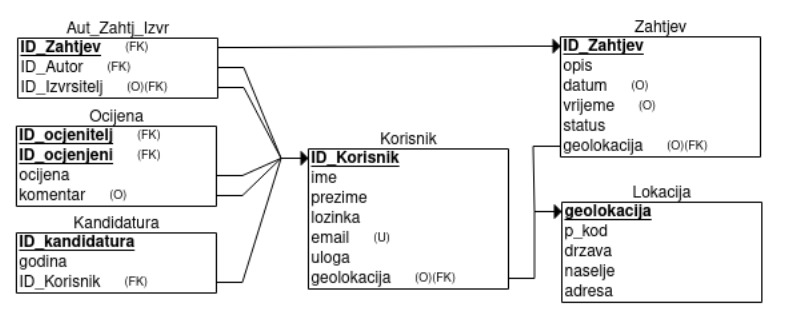
\includegraphics[scale=0.65]{slike/dijagram2.jpeg} %veličina slike u odnosu na originalnu datoteku i pozicija slike
				\centering
				\caption \newline E-R dijagram baze podataka
				\label{fig:promjene}
			\end{figure}
			
			\eject
			
			
		\section{Dijagram razreda}
		
			
			\textbf{\textit{dio 1. revizije}}\\
			
			\textit Na slikama 4.2, 4.3, 4.4 i 4.5 su prikazani dijagrami razreda za backend. Raspoređeni su u više slika radi bolje preglednosti i slične funkcionalnosti. Iz samih slika lakše se može uočiti povezanost samih stavki, njihova ovisnost te sadržaj atributa i funkcionalnosti.
			
			
			%unos slike
			\begin{figure}[H]
				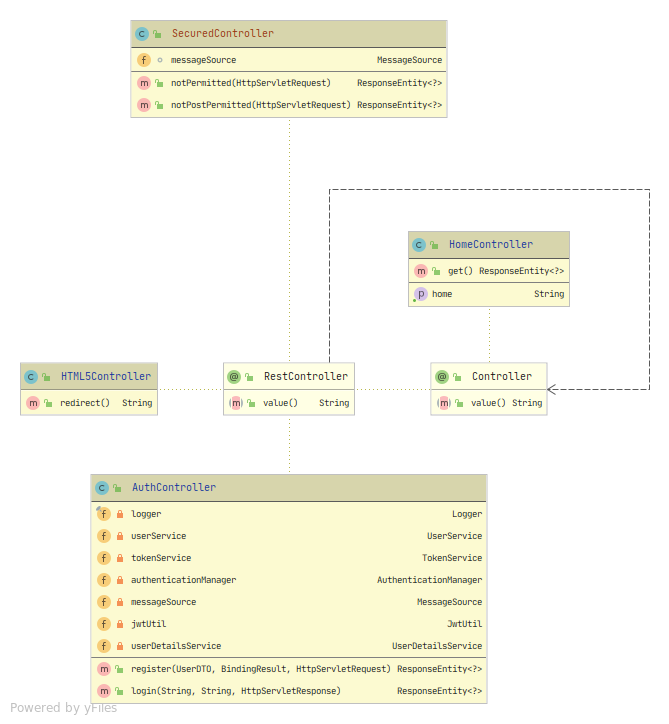
\includegraphics[scale=0.65]{slike/ControllersDiagram.png} %veličina slike u odnosu na originalnu datoteku i pozicija slike
				\centering
				\caption \newline Dijagram razreda za controllere
				\label{fig:promjene}
			\end{figure}
			
			%unos slike
			\begin{figure}[H]
				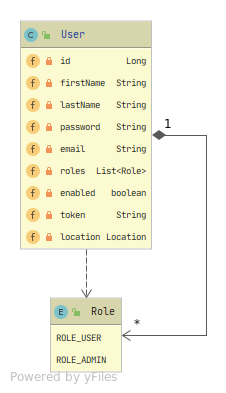
\includegraphics[scale=0.65]{slike/ModelUml.png} %veličina slike u odnosu na originalnu datoteku i pozicija slike
				\centering
				\caption \newline Dijagram razreda za model korisnika
				\label{fig:promjene}
			\end{figure}
			
			%unos slike
			\begin{figure}[H]
				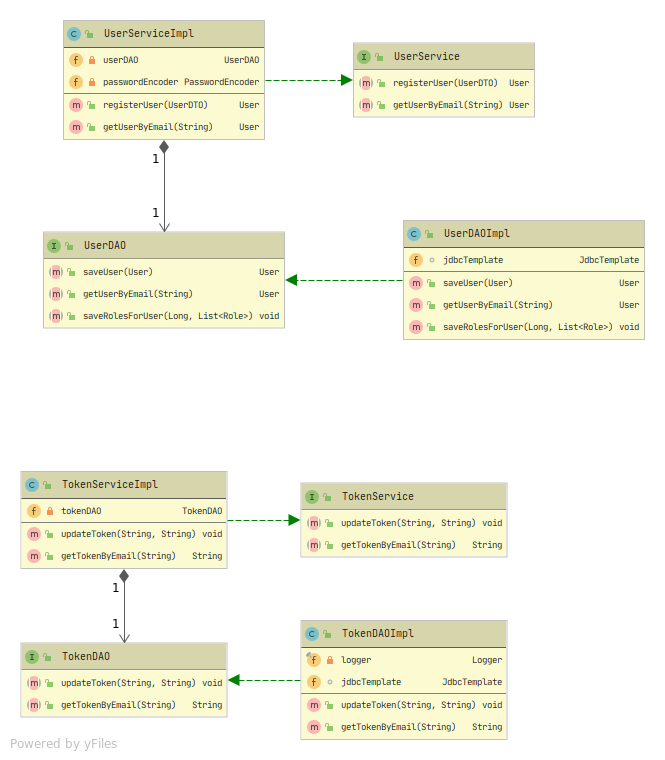
\includegraphics[scale=0.65]{slike/ServiceDaoUml.png} %veličina slike u odnosu na originalnu datoteku i pozicija slike
				\centering
				\caption \newline Dijagram razreda za ServiceDao
				\label{fig:promjene}
			\end{figure}
            
            %unos slike
			\begin{figure}[H]
				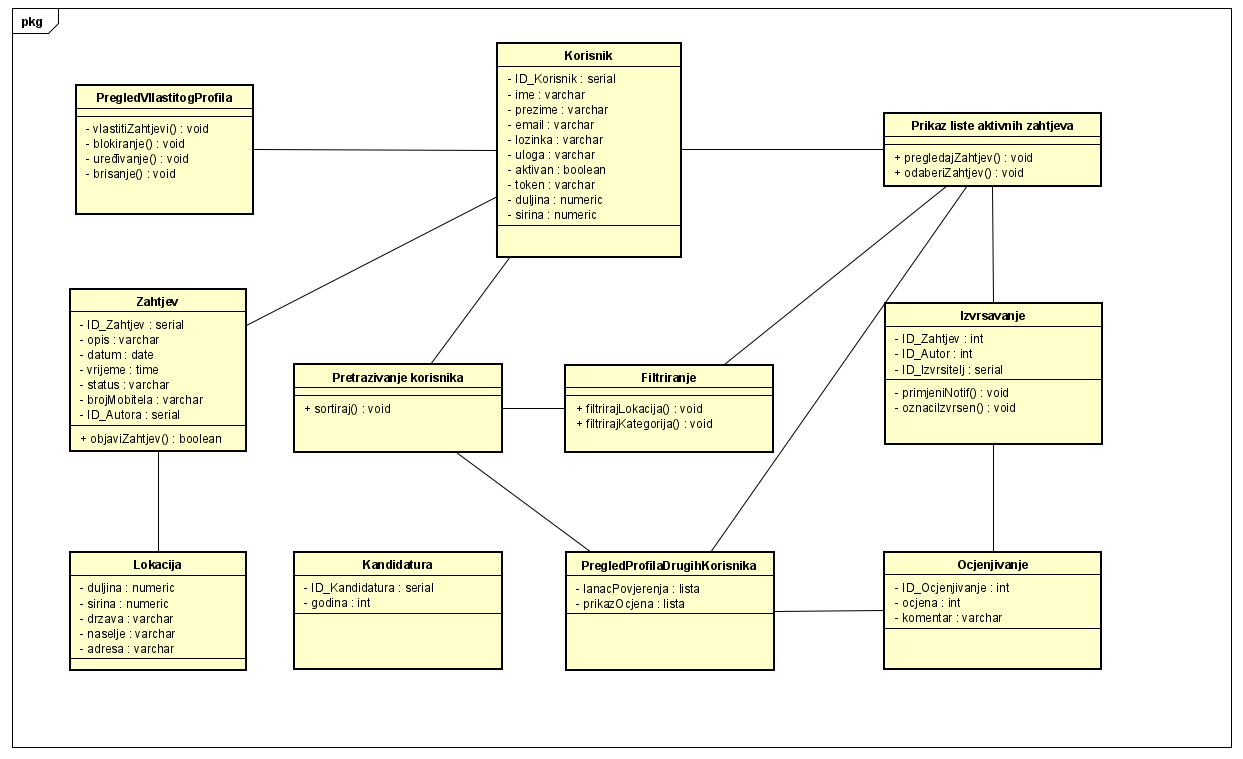
\includegraphics[scale=0.8]{slike/classDiagram1.png} %veličina slike u odnosu na originalnu datoteku i pozicija slike
				\centering
				\caption \newline Dijagram razreda - models
				\label{fig:promjene}
			\end{figure}
			 \begin{comment}
	\textbf{\textit{dio 2. revizije}}\\			
			
			
			\textit{Prilikom druge predaje projekta dijagram razreda i opisi moraju odgovarati stvarnom stanju implementacije}
			
			 \end{comment}

			
			\eject
		
		\section{Dijagram stanja}
			
			
			\textbf{\textit{dio 2. revizije}}\\
			
			\textit{Potrebno je priložiti dijagram stanja i opisati ga. Dovoljan je jedan dijagram stanja koji prikazuje \textbf{značajan dio funkcionalnosti} sustava. Na primjer, stanja korisničkog sučelja i tijek korištenja neke ključne funkcionalnosti jesu značajan dio sustava, a registracija i prijava nisu. }
			
			
			\eject 
		
		\section{Dijagram aktivnosti}
			
			\textbf{\textit{dio 2. revizije}}\\
			
			 \textit{Potrebno je priložiti dijagram aktivnosti s pripadajućim opisom. Dijagram aktivnosti treba prikazivati značajan dio sustava.}
			
			\eject
		\section{Dijagram komponenti}
		
			\textbf{\textit{dio 2. revizije}}\\
		
			 \textit{Potrebno je priložiti dijagram komponenti s pripadajućim opisom. Dijagram komponenti treba prikazivati strukturu cijele aplikacije.}